\documentclass[12pt,a4paper]{book}

% Fonts & Typography — Elegant and Professional
\usepackage[T1]{fontenc}
\usepackage{kpfonts} % Sleek, modern font
\usepackage{microtype}

% Essential Packages
\usepackage{graphicx}
\usepackage{fancyhdr}
\usepackage{tocloft}
\usepackage{titlesec}
\usepackage{datetime}
\usepackage{hyperref}
\usepackage{geometry}
\usepackage{parskip}
\usepackage{pgfplots}
\pgfplotsset{compat=1.18}
\usepackage{multicol} % Added for multicols environment

% Page Geometry — Slim, Clean Margins
\geometry{
  a4paper,
  left=10mm,
  right=10mm,
  top=20mm,
  bottom=20mm
}

% Header & Footer Styling
\pagestyle{fancy}
\fancyhf{}
\fancyhead[L]{\small \textit{\nouppercase{\leftmark}}}
\fancyhead[R]{\small K501: Quantative Analysis for Business Decisions}
\fancyfoot[C]{\small \thepage}
\renewcommand{\headrulewidth}{0.3pt}
\renewcommand{\footrulewidth}{0.3pt}

% Chapter Title Styling
\titleformat{\chapter}[block]
  {\normalfont\Huge\bfseries}
  {\thechapter.}{12pt}{}

\titleformat{\section}
  {\normalfont\Large\bfseries}
  {\thesection}{1em}{}

% Table of Contents Styling
\renewcommand{\cftchapfont}{\bfseries}
\renewcommand{\cftsecfont}{}
\setlength{\cftbeforechapskip}{5pt}
\setlength{\cftbeforesecskip}{2pt}
\setlength{\cftaftertoctitleskip}{1em}

% Hyperlink Styling
\hypersetup{
    colorlinks=true,
    linkcolor=blue,
    urlcolor=blue,
    pdftitle={K501: Quantative Analysis for Business Decisions},
    pdfpagemode=FullScreen,
}

% Custom Command for Notes 
\newcommand{\notesection}[2]{
  \section*{#1\\ \small \textit{#2}}
  \phantomsection
  \addcontentsline{toc}{section}{#1 - #2}
} 

% Document Start 
\begin{document}

% Title Page
\begin{titlepage}
    \centering
    \vspace*{3.5cm}
    
\includegraphics[width=0.28\textwidth]{logo.png}\par\vspace{1.5cm}
    {\scshape\LARGE University of Dhaka\par}
    \vspace{0.5cm}
    {\Large Institute of Business Administration (IBA)\par}
    \vspace{1.5cm}
    {\Huge\bfseries Master of Business Administration (MBA)\par}
    \vspace{1cm}
    {\Large K501: \textit{Quantative Analysis for Business Decision}\par}
    \vfill
    {\large Last Updated: \today\par}
\end{titlepage}

% Author Details Section 
\section*{Author Details}
\phantomsection
\addcontentsline{toc}{section}{Author Details}

\begin{center}
    \vspace{1em}
    \begin{tabular}{lll}
        \textbf{Name} & : & Md Hasibul Islam \\
        \textbf{Student ID} & : & 201-67-011 \\
        \textbf{Program} & : & Master of Business Administration (MBA) \\
        \textbf{Institute} & : & Institute of Business Administration (IBA) \\
        \textbf{University} & : & University of Dhaka \\
        \textbf{Email} & : & \href{mailto:hasiee8004@gmail.com}{hasiee8004@gmail.com} \\
        \textbf{LinkedIn} & : & \href{https://www.linkedin.com/in/hasib009}{linkedin.com/in/hasib009} \\
        \textbf{GitHub} & : & \href{https://github.com/HasibRockie}{github.com/HasibRockie} \\
        \textbf{Website} & : & \href{https://hasibrockie.github.io}{hasibrockie.github.io} \\
    \end{tabular}
    \vspace{1em}
\end{center}

\clearpage

% Table of Contents
\tableofcontents
\clearpage

% Notes Sections
\notesection{Statistics and Its Fundamental Concepts}{21-04-25 Monday}

\textbf{Statistics} is the science of collecting, organizing, analyzing, interpreting, and presenting data to support decision-making and problem-solving in business and other domains. It provides a quantitative foundation for managerial decisions by offering meaningful insights from data.

\vspace{0.5cm}
\textbf{Types of Statistics:}
\begin{enumerate}
    \item \textbf{Descriptive Statistics:} This involves methods of organizing, summarizing, and displaying data. 
    \begin{itemize}
        \item Examples: Mean, Median, Mode, Standard Deviation, Frequency tables, Pie charts, Histograms.
        \item Use Case: A retail manager summarizes last month's sales performance using a bar chart and average daily revenue.
    \end{itemize}

    \item \textbf{Inferential Statistics:} This refers to techniques for making generalizations from a sample to a population using probability theory.
    \begin{itemize}
        \item Examples: Hypothesis testing, Confidence intervals, Regression analysis.
        \item Use Case: A pharmaceutical company tests a new drug on a sample group to infer its effectiveness on the broader population.
    \end{itemize}
\end{enumerate}

\vspace{0.5cm}
\textbf{Types of Variables:}
\begin{itemize}
    \item \textbf{Qualitative (Categorical) Variables:} Represent categories or labels.
    \begin{itemize}
        \item Examples: Gender, Brand name, Type of customer (new/returning).
    \end{itemize}
    \item \textbf{Quantitative Variables:} Represent numeric values.
    \begin{itemize}
        \item \textbf{Discrete Variables:} Countable values (e.g., Number of employees).
        \item \textbf{Continuous Variables:} Measurable and can take any value within a range (e.g., Sales revenue, Temperature).
    \end{itemize}
\end{itemize}

\vspace{0.5cm}
\textbf{Levels of Measurement:}

\begin{table}[h!]
\centering
\resizebox{\textwidth}{!}{%
\begin{tabular}{|p{3cm}|p{5cm}|p{5cm}|p{5cm}|p{5cm}|}
\hline
\textbf{Characteristic} & \textbf{Nominal} & \textbf{Ordinal} & \textbf{Interval} & \textbf{Ratio} \\
\hline
\textbf{Definition} & 
Categorical data without any order & 
Categorical data with a logical order & 
Numeric data with equal intervals, no true zero & 
Numeric data with equal intervals and a true zero \\
\hline

\textbf{Nature of Data} & 
Labels or names & 
Ordered categories & 
Quantitative & 
Quantitative \\
\hline

\textbf{Mathematical Operations} & 
Equality only & 
Comparisons (>, <) & 
Addition, subtraction & 
All mathematical operations \\
\hline

\textbf{Meaningful Zero} & 
No & 
No & 
No & 
Yes \\
\hline

\textbf{Can Calculate Mean?} & 
No & 
No (median preferred) & 
Yes & 
Yes \\
\hline

\textbf{Examples} & 
Gender, Blood Type, Product Type & 
Socioeconomic Status, Education Level & 
Temperature (Celsius/Fahrenheit), IQ Score & 
Height, Weight, Age, Sales Revenue \\
\hline

\textbf{Applicable Statistics} & 
Mode, Frequency & 
Mode, Median, Percentile & 
Mean, SD, Correlation & 
All descriptive and inferential statistics \\
\hline

\textbf{Distance between values is meaningful?} & 
No & 
Not always & 
Yes & 
Yes \\
\hline

\textbf{Has absolute zero?} & 
No & 
No & 
No & 
Yes \\
\hline
\end{tabular}%
}
\caption{Comparison of Levels of Measurement}
\end{table}


\vspace{0.5cm}
\textbf{Other Key Concepts:}
\begin{itemize}
    \item \textbf{Population:} The entire group of individuals or instances about whom we hope to learn.
    \item \textbf{Sample:} A subset of the population, selected for analysis.
    \item \textbf{Parameter:} A numerical summary or measure that describes a characteristic of a population (e.g., population mean $\mu$).
    \item \textbf{Statistic:} A numerical summary derived from a sample (e.g., sample mean $\bar{x}$). Statistics are used to estimate parameters.
\end{itemize}

\vspace{2cm}

% new day 
\notesection{Classification of Variables with Examples}{28-04-25 Monday}

\textbf{Table 2: Classification of Variables — Qualitative vs Quantitative, Discrete vs Continuous}

\vspace{0.5cm}

\begin{table}[h!]
\centering
\begin{tabular}{|p{3cm}|p{7.5cm}|p{5.5cm}|}
\hline
\textbf{Variable Type} & \textbf{Discrete Examples} & \textbf{Continuous Examples} \\
\hline
\textbf{Qualitative } &
Shirt size (S, M, L) \newline
Product category (A, B, C) \newline
Number of children category (None, One, Two+) \newline
Room type (Single, Double) \newline
Education level (High School, UG, PG)
&
Skin tone spectrum \newline
Customer feedback scale \newline
Dialect variation \newline
Shade of color preferences \newline
Accent variation \\
\hline
\textbf{Quantitative} &
Number of cars owned \newline
Number of transactions \newline
Exam scores (out of 100) \newline
Number of employees \newline
Number of visits
&
Height (cm) \newline
Weight (kg) \newline
Income (\$) \newline
Temperature (°C) \newline
Time spent (hours) \\
\hline
\end{tabular}
\caption{Classification of Variables: Qualitative vs Quantitative and Discrete vs Continuous}
\end{table}
    
\vspace{1cm}

\textbf{Table 3: Classification by Levels of Measurement — Nominal, Ordinal, Interval, Ratio with Discrete and Continuous Types}

\vspace{0.3cm}

\begin{table}[h!]
\centering

\begin{tabular}{|p{3cm}|p{6cm}|p{6cm}|}
\hline
\textbf{Level of Measurement} & \textbf{Discrete Examples} & \textbf{Continuous Examples} \\
\hline
\textbf{Nominal} &
\begin{itemize}
    \item Jersey number
    \item Postal code
    \item Nationality
    \item Product ID
    \item Car model
\end{itemize}
&
\begin{itemize}
    \item Color shade
    \item Accent pattern
    \item Logo design variation
    \item Pattern of speech
    \item Ink density
\end{itemize}
\\
\hline
\textbf{Ordinal} &
\begin{itemize}
    \item Customer rating (1–5 stars)
    \item Survey rank (Strongly disagree to Agree)
    \item Academic grade (A, B, C)
    \item Job level (Junior, Mid, Senior)
    \item Market tier (Low, Mid, High)
\end{itemize}
&
\begin{itemize}
    \item Satisfaction level on 0–10 scale
    \item Credit score bands
    \item Health condition severity
    \item Employee performance level
    \item Risk tolerance scale
\end{itemize}
\\
\hline
\textbf{Interval} &
\begin{itemize}
    \item Test scores (e.g., IQ, SAT)
    \item Temperature recorded hourly
    \item Credit scores in discrete brackets
    \item Year of birth
    \item Calendar dates
\end{itemize}
&
\begin{itemize}
    \item Temperature (°C or °F)
    \item Time of day (without AM/PM)
    \item Financial index points
    \item Sound intensity
    \item Wind speed variation
\end{itemize}
\\
\hline
\textbf{Ratio} &
\begin{itemize}
    \item Number of products sold
    \item Number of goals scored
    \item Number of books owned
    \item Defect counts in production
    \item Visitors per day
\end{itemize}
&
\begin{itemize}
    \item Income
    \item Distance traveled
    \item Weight
    \item Time
    \item Age
\end{itemize}
\\
\hline
\end{tabular}

\caption{50 Examples Categorized by Level of Measurement and Variable Type}
\end{table}

\vspace{1cm}
\clearpage

\notesection{Classification of Interval and Ratio Data}{05-05-25 Monday}

\textbf{Table 1: Examples of Interval vs Ratio Data}

\vspace{0.5cm}

\begin{table}[h!]
\centering
\begin{tabular}{|p{8cm}|p{8cm}|}
\hline
\textbf{Interval Examples} & \textbf{Ratio Examples} \\
\hline
Temperature (°C or °F) & Height (cm) \\
IQ scores & Weight (kg) \\
Calendar years (e.g., 1990, 2000) & Income (\$) \\
Time of day (without AM/PM) & Distance (miles, km) \\
Standardized test scores (e.g., SAT) & Age (years) \\
Body temperature (°C or °F) & Speed (km/h, m/s) \\
Elevation (altitude above sea level) & Amount of money in a bank account (\$) \\
Scores on a thermometer (not Celsius) & Number of products produced \\
Electrical voltage (in volts) & Number of hours worked \\
Sea level pressure in hPa & Time spent on an activity (minutes, hours) \\
Temperature difference (relative to a baseline) & Volume of water in a tank (liters) \\
Time intervals (measured in minutes, seconds) & Weight of an object (kg) \\
Age difference between two people (in years) & Height of a building (meters) \\
Test scores in degrees (e.g., temperature degrees in a test) & Distance traveled (km) \\
Time elapsed (counted in minutes or hours) & Duration of an event (seconds, hours) \\
Yearly income (adjusted for inflation) & Car mileage (km per liter) \\
Currency fluctuation in a day & Number of children in a family \\
Dates in history (e.g., 1776, 2000) & Average monthly rent (\$) \\
Income tax (as a percentage of income) & Calories burned (kcal) \\
Temperature increase over a day & Amount of rainfall (cm) \\
Time difference in hours (e.g., time zones) & Number of cups of coffee consumed \\
Survey scores (e.g., 1 to 10 scale) & Blood pressure level (mm Hg) \\
Duration in seconds (e.g., a stopwatch) & Quantity of goods sold \\
Difference in height between two points on Earth & Quantity of raw material processed \\
Height of a mountain (in meters) & Hours of sleep per night \\
\hline
\end{tabular}
\caption{Examples of Interval and Ratio Data}
\end{table}

\vspace{1cm}

\textbf{Table 2: Continuous vs Discrete Examples for Interval and Ratio Data}

\vspace{0.5cm}

\begin{table}[h!]
\centering
\begin{tabular}{|p{8cm}|p{8cm}|}
\hline
\textbf{Continuous Examples} & \textbf{Discrete Examples} \\
\hline
Temperature (°C or °F) & Number of children in a family \\
Height (cm) & Number of cars owned \\
Weight (kg) & Number of transactions made \\
Age (years) & Number of goals scored in a game \\
Distance (miles, km) & Number of students in a class \\
Speed (km/h, m/s) & Number of employees in a company \\
Time spent on a task (minutes, hours) & Number of books in a library \\
Amount of money in a bank account (\$) & Number of visitors to a website \\
Volume of water in a tank (liters) & Number of rooms in a house \\
Duration of an event (seconds, minutes) & Number of items sold in a day \\
Calories burned (kcal) & Number of people in a line \\
Amount of rainfall (cm) & Number of phone calls received \\
Number of cups of coffee consumed & Number of hours worked per week \\
Blood pressure level (mm Hg) & Number of students passing an exam \\
Height of a building (meters) & Number of cars in a parking lot \\
Hours of sleep per night & Number of pets owned \\
Monthly rent (\$) & Number of emails sent in a day \\
Total income for the year (\$) & Number of tickets sold for an event \\
Survey scores (e.g., 1 to 10 scale) & Number of products produced in a factory \\
Time intervals (measured in minutes) & Number of patients in a hospital \\
Test scores (standardized) & Number of questions answered correctly on a quiz \\
Time difference between locations (e.g., time zone differences) & Number of units produced per hour \\
Total calories consumed in a day & Number of visitors to a museum \\
Survey feedback score (1 to 10) & Number of cups in a cupboard \\
Time elapsed in hours (e.g., work hours) & Number of toys in a box \\
\hline
\end{tabular}
\caption{Continuous vs Discrete Examples for Interval and Ratio Data}
\end{table}

\vspace{1cm}
\clearpage


\notesection{Frequency Distribution and Mean Classifications}{12-05-25 Thursday}

\textbf{Frequency Distribution and Parameters}

\vspace{0.5cm}

\textbf{Frequency Distribution:}
A frequency distribution is a table that displays the frequency (i.e., how often each value appears) of different values or categories in a dataset. It helps to organize and summarize data, providing insight into the underlying patterns.

\vspace{0.5cm}
\textbf{Parameters of Frequency Distribution:}

\begin{itemize}
    \item \textbf{k (Number of Classes):} The number of categories or intervals that data will be grouped into. It is typically chosen based on the range and size of the dataset.
    \item \textbf{N (Total Number of Data Points):} The total number of observations or data points in the dataset.
    \item \textbf{i (Class Width):} The width of each class interval, calculated using the formula:
    \[
    i = \frac{\text{Max} - \text{Min}}{k}
    \]
    where \(\text{Max}\) and \(\text{Min}\) represent the maximum and minimum values in the dataset, respectively.
    \item The rule for selecting \(k\) is: \(2^k > N\), where \(k\) is the number of classes, and \(N\) is the total number of observations.
\end{itemize}

\vspace{0.5cm}
\textbf{Example:}
Suppose you have a dataset of 50 data points (\(N = 50\)), and the range of the data is from 10 to 100.

To determine the number of classes (\(k\)) and the class width (\(i\)):

\[
2^k > 50 \quad \Rightarrow \quad k = 6 \quad \text{(as } 2^6 = 64 > 50\text{)}
\]

\[
i = \frac{100 - 10}{6} = 15
\]

Thus, the number of classes \(k\) will be 6, and each class will have a width of 15.

\vspace{1cm}

\textbf{Mean}

\vspace{0.5cm}

\textbf{1. Arithmetic Mean:}
The arithmetic mean, commonly referred to as the average, is the sum of all values in the dataset divided by the number of values. It is the most widely used measure of central tendency.

\[
\text{Arithmetic Mean} (\bar{x}) = \frac{\sum x}{N}
\]
Where:
- \(x\) represents each data point,
- \(N\) is the number of data points.

\textbf{Example:}
For the dataset: 2, 4, 6, 8, 10,
\[
\bar{x} = \frac{2 + 4 + 6 + 8 + 10}{5} = \frac{30}{5} = 6
\]

\vspace{0.5cm}

\textbf{2. Geometric Mean:}
The geometric mean is the nth root of the product of all values in a dataset, where \(n\) is the number of values. The geometric mean is often used when comparing values that have different ranges, such as growth rates.

\[
\text{Geometric Mean} (GM) = \left( \prod_{i=1}^{N} x_i \right)^{\frac{1}{N}}
\]
Where:
- \(x_i\) represents each data point,
- \(N\) is the number of data points.

\textbf{Example:}
For the dataset: 1, 4, 16, 64,
\[
GM = (1 \times 4 \times 16 \times 64)^{\frac{1}{4}} = 1024^{\frac{1}{4}} = 8
\]

\vspace{0.5cm}

\textbf{3. Weighted Mean:}
The weighted mean is a variation of the arithmetic mean where each data point is assigned a weight that reflects its importance or frequency. The weighted mean is particularly useful when some values in the dataset are more significant than others.

\[
\text{Weighted Mean} = \frac{\sum w_i x_i}{\sum w_i}
\]
Where:
- \(w_i\) is the weight associated with data point \(x_i\),
- \(x_i\) is the value of the data point,
- \(N\) is the total number of data points.

\textbf{Example:}
For the dataset: (value, weight): \((2, 3), (4, 2), (6, 5)\),
\[
\text{Weighted Mean} = \frac{(3 \times 2) + (2 \times 4) + (5 \times 6)}{3 + 2 + 5} = \frac{6 + 8 + 30}{10} = \frac{44}{10} = 4.4
\]

\vspace{1cm}


\textbf{Mode, Median, and Common Measures of Location}

\vspace{0.5cm}

\textbf{1. Mode:} \\
The mode is the value that appears most frequently in a data set. It is the only measure of central tendency that can be used for nominal data. A dataset may have no mode, one mode (unimodal), or multiple modes (bimodal or multimodal).

\textbf{Example:} \\
For the dataset: 3, 3, 4, 5, 6, 6, 6, 7, \\
- Mode = 6 (appears most frequently).

\vspace{0.5cm}

\textbf{2. Median:} \\
The median is the middle value when the data is arranged in ascending or descending order. If the number of data points is odd, the median is the middle number. If it is even, the median is the average of the two middle numbers.

\textbf{Example:} \\
For the dataset: 1, 3, 5, 7, 9, \\
- Median = 5 (middle value).

For the dataset: 1, 3, 5, 7, \\
- Median = (3 + 5) / 2 = 4.

\vspace{0.5cm}

\textbf{3. Other Measures of Location:} \\
In addition to the mode and median, other measures of location include the mean (discussed earlier), quartiles, and percentiles, which divide the data into specific parts:
- Quartiles split data into four equal parts.
- Percentiles divide the data into 100 equal parts, useful for detailed analysis.

---

\subsection*{Population Mean and Sample Mean}

\vspace{0.5cm}

\textbf{Population Mean:} \\
The population mean (\(\mu\)) is the average of all the values in the population. It is calculated by summing all the values and dividing by the total number of values in the population.

\[
\mu = \frac{\sum x_i}{N}
\]

Where:
- \(x_i\) represents each individual data point,
- \(N\) is the total number of data points in the population.

\textbf{Example:} \\
For the population data: 2, 4, 6, 8, 10, \\
\[
\mu = \frac{2 + 4 + 6 + 8 + 10}{5} = \frac{30}{5} = 6
\]

\vspace{0.5cm}

\textbf{Sample Mean:} \\
The sample mean (\(\bar{x}\)) is the average of a sample taken from the population. It is calculated in the same way as the population mean but uses the sample data.

\[
\bar{x} = \frac{\sum x_i}{n}
\]

Where:
- \(x_i\) represents each individual data point in the sample,
- \(n\) is the number of data points in the sample.

\textbf{Example:} \\
For the sample data: 1, 3, 5, 7, 9, \\
\[
\bar{x} = \frac{1 + 3 + 5 + 7 + 9}{5} = \frac{25}{5} = 5
\]

\vspace{1cm} 

\notesection{Measures of Dispersion and Range}{10-04-25 Thursday}

\textbf{Dispersion and Range}

\vspace{0.5cm}

\textbf{1. Dispersion:}
Dispersion refers to the extent to which a distribution is spread out. Common measures of dispersion include:
- **Range**
- **Variance**
- **Standard deviation**

\textbf{2. Range:}
The range is the difference between the maximum and minimum values in a dataset.

\[
\text{Range} = \text{Max} - \text{Min}
\]

\textbf{Example:}
For the dataset: 2, 4, 6, 8, 10, the range is:
\[
\text{Range} = 10 - 2 = 8
\]


\begin{figure}[h!]  % Optional: Use the 'figure' environment for better positioning
\centering
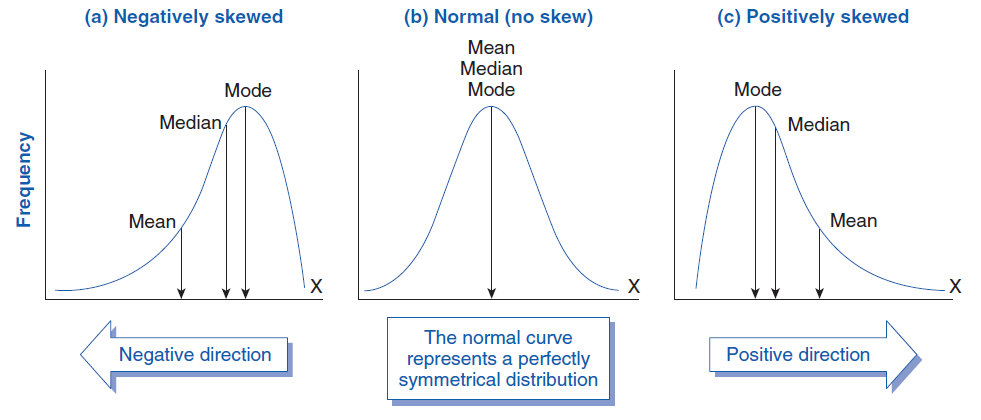
\includegraphics[width=\textwidth]{imgs/distribution.png}
\caption{Distribution (a) Negatively skewed, (b) symmetric, (c) Positively Skewed}  
\end{figure}

\vspace{1cm}

\textbf{Variance and Standard Deviation}

\vspace{0.5cm}

\textbf{1. Variance:} \\
Variance is a measure of the spread between numbers in a dataset. It quantifies the average squared deviation from the mean. A larger variance indicates that the data points are more spread out from the mean.

\[
\text{Variance (Population)} = \sigma^2 = \frac{1}{N} \sum_{i=1}^{N} (x_i - \mu)^2
\]

Where:
\begin{itemize}
    \item \( \sigma^2 \) is the population variance,
    \item \( x_i \) is each data point,
    \item \( \mu \) is the population mean,
    \item \( N \) is the total number of data points.
\end{itemize}

\textbf{Example:} \\
For the population data: 4, 7, 8, 5, 9 \\
Mean \( \mu = \frac{4 + 7 + 8 + 5 + 9}{5} = 6.6 \) \\
Variance \( \sigma^2 = \frac{(4-6.6)^2 + (7-6.6)^2 + (8-6.6)^2 + (5-6.6)^2 + (9-6.6)^2}{5} = 3.04 \)

\vspace{0.5cm}

\textbf{2. Standard Deviation:} \\
Standard deviation is the square root of variance and gives a measure of the spread in the same units as the data. It is used when we need a value that directly describes the data's variability.

\[
\text{Standard Deviation (Population)} = \sigma = \sqrt{\frac{1}{N} \sum_{i=1}^{N} (x_i - \mu)^2}
\]

\textbf{Example:} \\
For the population data: 4, 7, 8, 5, 9 \\
Standard deviation \( \sigma = \sqrt{3.04} = 1.74 \)

\vspace{0.5cm}

\textbf{Use Cases:}
\begin{itemize}
    \item \textbf{Variance} is primarily used in statistical analysis, particularly when comparing data sets with different units or when further statistical procedures are needed (e.g., ANOVA, regression analysis).
    \item \textbf{Standard Deviation} is commonly used in real-world applications where data spread or variability is crucial, such as finance (e.g., measuring stock price fluctuations) or quality control (e.g., measuring consistency in manufacturing).
\end{itemize}

---

\textbf{Degree of Freedom and Its Implications}

\vspace{0.5cm}

\textbf{Degree of Freedom (df):} \\
Degrees of freedom refer to the number of independent values or quantities that can vary in an analysis without violating any given constraints. It is crucial in statistical tests (e.g., t-tests, chi-square tests), as it determines the appropriate distribution for hypothesis testing.

For a sample, the degrees of freedom for variance and standard deviation are given by:

\[
\text{Variance (Sample)} = \frac{1}{n-1} \sum_{i=1}^{n} (x_i - \bar{x})^2
\]

Where:
\begin{itemize}
    \item \( \bar{x} \) is the sample mean,
    \item \( n \) is the sample size,
    \item \( n-1 \) is the degrees of freedom.
\end{itemize}

The reason for using \( n-1 \) instead of \( n \) is to account for the \textbf{bias} in the estimate of population variance when using a sample.

\textbf{Implication of Degrees of Freedom:}
\begin{itemize}
    \item The \textbf{degrees of freedom} in a sample determine the \textbf{accuracy of statistical estimates}. Reducing the degrees of freedom (i.e., increasing the number of constraints) reduces the variability of the sample estimate, making it more reliable.
    \item In the context of hypothesis testing, the degrees of freedom affect the \textbf{critical value} used to assess whether the observed statistic is significant.
\end{itemize}

\textbf{Example:}
For the sample data: 4, 7, 8, 5, 9 (sample size \(n = 5\)) \\
Degrees of freedom \(df = n - 1 = 5 - 1 = 4\)
 
\vspace{2cm}


\notesection{Solving Statistics in Excel: Mean, Mode, Median, Variance, and Standard Deviation}{12-05-25 Monday}

\textbf{1. Mean (Average):}

\vspace{0.5cm}

\textbf{Excel Function:} \\
The \texttt{AVERAGE} function is used to calculate the mean of a dataset in Excel.

\[
\texttt{=AVERAGE(range)}
\]

Where:
- \texttt{range} is the range of data points you want to calculate the mean for.

\textbf{Use Case:}
- Used to find the central tendency of the dataset.

\textbf{Example:}
For the dataset: 4, 7, 8, 5, 9, the formula would be:

\[
\texttt{=AVERAGE(4, 7, 8, 5, 9)} \rightarrow 6.6
\]
\[
\texttt{=AVERAGE(A2:A20)}
\]


\textbf{2. Mode (Most Frequent Value):}

\vspace{0.5cm}

\textbf{Excel Function:} \\
The \texttt{MODE} function is used to find the most frequent number in a dataset.

\[
\texttt{=MODE(range)}
\]

Where:
- \texttt{range} is the dataset you are analyzing.

\textbf{Use Case:}
- Used when you want to find the most common or frequent data point in a set.

\textbf{Example:}
For the dataset: 3, 3, 4, 5, 6, 6, 6, the formula would be:

\[
\texttt{=MODE(3, 3, 4, 5, 6, 6, 6)} \rightarrow 6
\]
\[
\texttt{=MODE(A2:A20)}
\]


\textbf{3. Median (Middle Value):}

\vspace{0.5cm}

\textbf{Excel Function:} \\
The \texttt{MEDIAN} function is used to calculate the middle value of a dataset when the data is arranged in ascending or descending order.

\[
\texttt{=MEDIAN(range)}
\]

Where:
- \texttt{range} is the dataset from which the median will be calculated.

\textbf{Use Case:}
- Used when the data has outliers or is skewed, as it gives the middle value that separates the higher half from the lower half.

\textbf{Example:}
For the dataset: 1, 3, 5, 7, 9, the formula would be:

\[
\texttt{=MEDIAN(1, 3, 5, 7, 9)} \rightarrow 5
\]

For an even number of values (1, 3, 5, 7), the formula would return the average of the two middle values:

\[
\texttt{=MEDIAN(1, 3, 5, 7)} \rightarrow 4
\]

---

\textbf{4. Variance (Measure of Spread):}

\vspace{0.5cm}

\textbf{Excel Functions:} \\
- For \textbf{population variance}, use the \texttt{VAR.P} function.
  
\[
\texttt{=VAR.P(range)}
\]

- For \textbf{sample variance}, use the \texttt{VAR.S} function.

\[
\texttt{=VAR.S(range)}
\]

Where:
- \texttt{VAR.P} is used for data representing an entire population.
- \texttt{VAR.S} is used for data representing a sample of a population.

\textbf{Use Case:}
- \texttt{VAR.P} is used when you have data for an entire population, and \texttt{VAR.S} is used when you have a sample of data.

\textbf{Example:}
For the dataset (Population): 4, 7, 8, 5, 9, the formula for \textbf{population variance} would be:

\[
\texttt{=VAR.P(4, 7, 8, 5, 9)} \rightarrow 3.04
\]

For the dataset (Sample): 4, 7, 8, 5, 9, the formula for \textbf{sample variance} would be:
 
\[
\texttt{=VAR.S(4, 7, 8, 5, 9)} \rightarrow 3.8
\]

---

\textbf{5. Standard Deviation (Measure of Spread in the Same Units):}

\vspace{0.5cm}

\textbf{Excel Functions:} \\
- For \textbf{population standard deviation}, use the \texttt{STDEV.P} function.
  
\[
\texttt{=STDEV.P(range)}
\]

- For \textbf{sample standard deviation}, use the \texttt{STDEV.S} function.

\[
\texttt{=STDEV.S(range)}
\]

Where:
- \texttt{STDEV.P} is used for data representing an entire population.
- \texttt{STDEV.S} is used for data representing a sample of a population.

\textbf{Use Case:}
- Standard deviation is used when you want a measure of spread in the same units as the data.

\textbf{Example:}
For the dataset (Population): 4, 7, 8, 5, 9, the formula for \textbf{population standard deviation} would be:

\[
\texttt{=STDEV.P(4, 7, 8, 5, 9)} \rightarrow 1.74
\]

For the dataset (Sample): 4, 7, 8, 5, 9, the formula for \textbf{sample standard deviation} would be:

\[
\texttt{=STDEV.S(4, 7, 8, 5, 9)} \rightarrow 1.95
\]

---

\textbf{Summary of Functions:}

\begin{itemize}
    \item \texttt{AVERAGE(range)}: Mean of the data.
    \item \texttt{MODE(range)}: Mode (Most frequent value) of the data.
    \item \texttt{MEDIAN(range)}: Median (Middle value) of the data.
    \item \texttt{VAR.P(range)}: Population variance.
    \item \texttt{VAR.S(range)}: Sample variance.
    \item \texttt{STDEV.P(range)}: Population standard deviation.
    \item \texttt{STDEV.S(range)}: Sample standard deviation.
\end{itemize}

\clearpage 

\textbf{1. Bar Chart:}

\vspace{0.5cm}

\textbf{Use Case:} \\
Bar charts are useful for comparing the frequencies, values, or categories of data. They are typically used when you want to compare data across different categories.

\textbf{Creating a Bar Chart in Excel:}
\begin{itemize}
    \item Highlight the data range (including headers).
    \item Go to the "Insert" tab.
    \item Click on "Bar Chart" and select the type of bar chart you want (e.g., Clustered Bar, Stacked Bar, etc.).
\end{itemize}

\textbf{Example:} \\
Suppose you have sales data for different products:
\[
\begin{array}{|c|c|}
\hline
\text{Product} & \text{Sales} \\
\hline
\text{Product A} & 300 \\
\text{Product B} & 450 \\
\text{Product C} & 200 \\
\hline
\end{array}
\]

A bar chart will display the products on the x-axis and the sales on the y-axis, visually comparing their sales.

---

\textbf{2. Histogram:}

\vspace{0.5cm}

\textbf{Use Case:} \\
Histograms are used to show the distribution of numerical data. They are particularly useful for understanding the frequency of values within a certain range.

\textbf{Creating a Histogram in Excel:}
\begin{itemize}
    \item Select the data for which you want to create a histogram.
    \item Go to the "Insert" tab.
    \item Click "Insert Statistic Chart" and select "Histogram."
    \item Excel will automatically group the data into bins.
\end{itemize}

\textbf{Example:} \\
If you have test scores for 10 students:
\[
\text{Scores: } 75, 80, 85, 88, 90, 92, 85, 76, 91, 94
\]

The histogram will show how many students fall within each score range (e.g., 70-80, 81-90, 91-100).

---

\textbf{3. Column Chart:}

\vspace{0.5cm}

\textbf{Use Case:} \\
Column charts are similar to bar charts but are oriented vertically. They are commonly used to compare data across categories and to visualize trends over time (e.g., monthly sales data).

\textbf{Creating a Column Chart in Excel:}
\begin{itemize}
    \item Highlight the data range (including headers).
    \item Go to the "Insert" tab.
    \item Click "Column Chart" and choose the chart type (e.g., Clustered Column, Stacked Column).
\end{itemize}

\textbf{Example:} \\
If you have quarterly revenue data:
\[
\begin{array}{|c|c|}
\hline
\text{Quarter} & \text{Revenue} \\
\hline
\text{Q1} & 5000 \\
\text{Q2} & 7000 \\
\text{Q3} & 8000 \\
\text{Q4} & 6000 \\
\hline
\end{array}
\]

The column chart will display the revenue for each quarter, allowing easy comparison.

---

\textbf{4. Line Chart:}

\vspace{0.5cm}

\textbf{Use Case:} \\
Line charts are ideal for displaying trends over time, such as stock prices, sales over months, or other time-based data.

\textbf{Creating a Line Chart in Excel:}
\begin{itemize}
    \item Highlight the data range (including headers).
    \item Go to the "Insert" tab.
    \item Click on "Line Chart" and choose the chart type (e.g., Line, Stacked Line).
\end{itemize}

\textbf{Example:} \\
For a dataset representing monthly temperatures:
\[
\begin{array}{|c|c|}
\hline
\text{Month} & \text{Temperature (°C)} \\
\hline
\text{January} & 5 \\
\text{February} & 6 \\
\text{March} & 10 \\
\text{April} & 15 \\
\text{May} & 20 \\
\hline
\end{array}
\]

A line chart will show how the temperature increases over the months.

---

\textbf{5. Pie Chart:}

\vspace{0.5cm}

\textbf{Use Case:} \\
Pie charts are used to show the proportions of a whole. They are ideal for showing percentages or proportions of a category in a dataset.

\textbf{Creating a Pie Chart in Excel:}
\begin{itemize}
    \item Highlight the data range (including headers).
    \item Go to the "Insert" tab.
    \item Click on "Pie Chart" and select the type of pie chart you want (e.g., 2-D Pie, 3-D Pie).
\end{itemize}

\textbf{Example:} \\
If you have market share data for four companies:
\[
\begin{array}{|c|c|}
\hline
\text{Company} & \text{Market Share} \\
\hline
\text{Company A} & 40\% \\
\text{Company B} & 30\% \\
\text{Company C} & 20\% \\
\text{Company D} & 10\% \\
\hline
\end{array}
\]

A pie chart will show the proportion of the market share for each company.

---

\textbf{6. Scatter Plot:}

\vspace{0.5cm}

\textbf{Use Case:} \\
Scatter plots are used to display relationships between two variables. They are useful for showing correlations or the lack thereof.

\textbf{Creating a Scatter Plot in Excel:}
\begin{itemize}
    \item Highlight the data range (including headers).
    \item Go to the "Insert" tab.
    \item Click "Scatter Plot" and select the type of scatter chart you want (e.g., Simple Scatter, Scatter with Lines).
\end{itemize}

\textbf{Example:} \\
If you have the data for advertising spend and sales revenue:
\[
\begin{array}{|c|c|}
\hline
\text{Advertising Spend} & \text{Sales Revenue} \\
\hline
1000 & 5000 \\
2000 & 7000 \\
3000 & 9000 \\
4000 & 11000 \\
\hline
\end{array}
\]

A scatter plot will display the relationship between advertising spend and sales revenue, helping to identify trends or correlations.

\vspace{1cm} 

\textbf{Conclusion:}

In Excel, different chart types serve distinct purposes:
\begin{itemize}
    \item \textbf{Bar Charts}: Compare categories or values.
    \item \textbf{Histograms}: Show the distribution of numerical data.
    \item \textbf{Column Charts}: Compare data across categories or trends over time.
    \item \textbf{Line Charts}: Display trends or changes over time.
    \item \textbf{Pie Charts}: Show proportions of a whole.
    \item \textbf{Scatter Plots}: Show relationships between two variables.
\end{itemize}

These charts are fundamental tools for visual data analysis and are used depending on the type of data and the analysis you want to perform.

\vspace{1cm}
\clearpage 

% new note 
\notesection{2025-04-23}{Wednesday}
\textbf{Topics Covered:}

\clearpage

% end of the note 


\end{document}
